\documentclass{article}
\usepackage[utf8]{inputenc}
\usepackage[export]{adjustbox}
\usepackage{subfig}
\usepackage{graphicx}
\usepackage{wrapfig}
\graphicspath {
	{images/}
}

\begin{document}

\title{Design Ideas}
\author{Cardspark - Group 26}
\date{\today}
\maketitle

We took the problems that we had found through our research of our target audience and undertook the process of generating ideas.
The following are the problems or wants had by our users and how we tried to solve them:
\vspace{-2mm}

\paragraph{\textbf{- That solution notes are often too large and difficult to consume}}
	\mbox{}\\
	We looked around at other apps and saw different ways of dealing with large amounts of information.
	\begin{figure}[!ht]
	  \centering
	  \subfloat{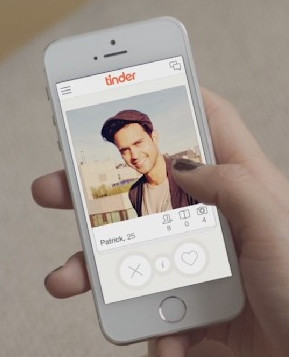
\includegraphics[scale=0.4]{tinder.jpg}\label{fig:f1}}
	  \hfill
	  \subfloat{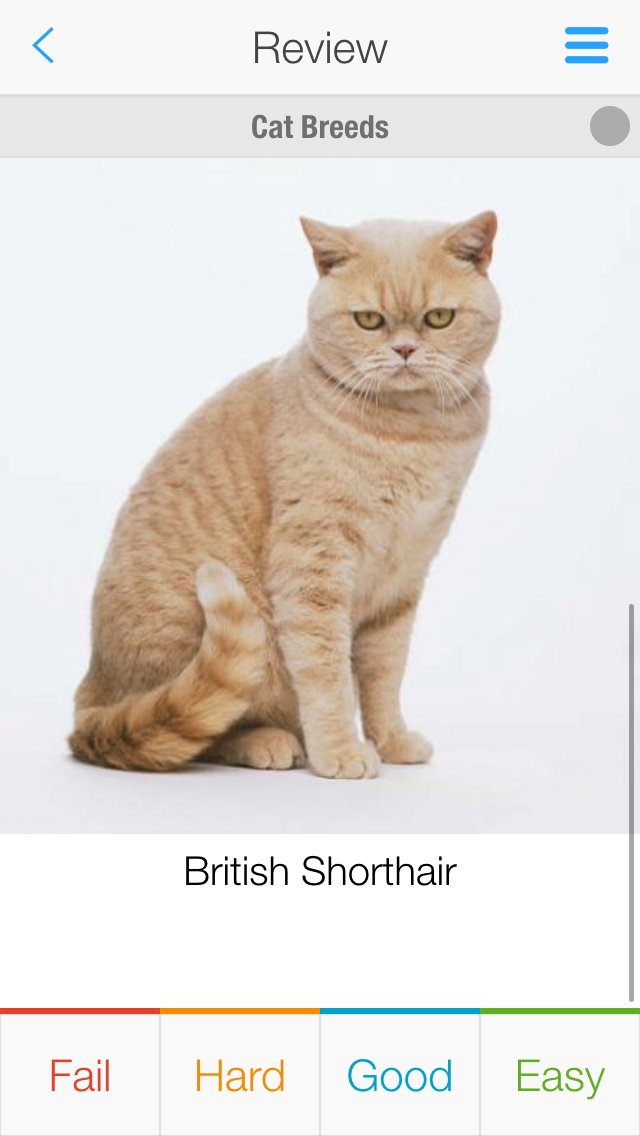
\includegraphics[scale=0.13]{anki.png}\label{fig:f2}}
	\end{figure}
	\\Tinder (above left) deals with the thousands of possible "matches" a person has to scroll through by using a swiping mechanism. Anki (above right) is a flash card that requires the user to provide a response to a flashcard.  We decided to go with the swiping option to allow the user more manipulation of their cards.
\newpage

\paragraph{\textbf{- There were not enough opportunities for group work in learning}}
	\mbox{}\\
	\begin{figure}[!ht]
	  \centering
	  \subfloat{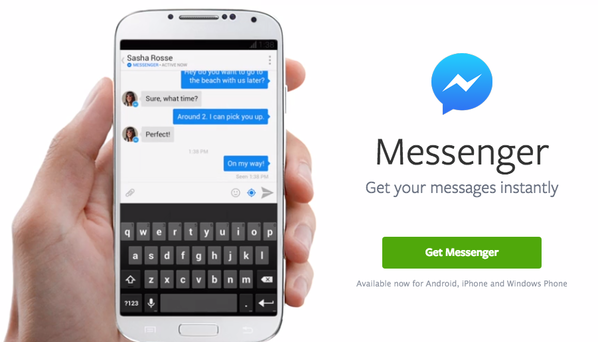
\includegraphics[scale=0.35]{messenger.png}\label{fig:f4}}
	\end{figure}
	\\We investigated mobile apps like Messenger that focused on group features, in that case communication.  We wanted to transfer this idea of collaboration to Cardspark by allowing multiple people to create flashcards and then share them, almost like the messages in Messenger.

\vspace{5mm}
\paragraph{\textbf{- That testing themselves was an important part of the learning process for them}}
	\mbox{}\\
	\begin{figure}[!ht]
	  \centering
	  \subfloat{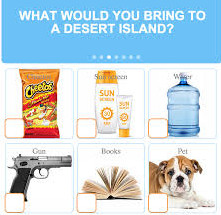
\includegraphics[scale=0.5]{buzzfeed.jpg}\label{fig:f5}}
	  \hfill
	  \subfloat{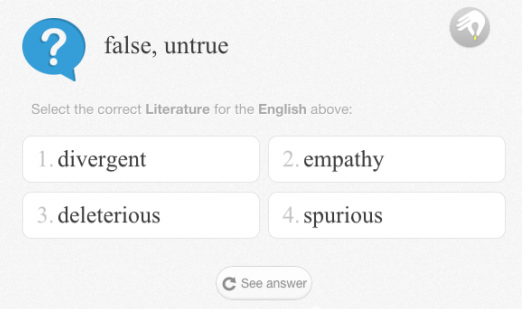
\includegraphics[scale=0.35]{memrise.png}\label{fig:f6}}
	\end{figure}
	\\The testing feature that was wanted was inspired by Memrise's (language app) and to an extent Buzzfeed's quiz.  Buzzfeed's quiz feature shares the multi-choice functionality of Memrise so we saw this as a good idea for our own quiz system.

\vspace{5mm}
\paragraph{\textbf{- Visual cues like images and colours were very helpful to them}}
	\mbox{}\\
	We, again, took inspiration from Tinder for their image placement and how it shows that they could be used well in a card format.  Buzzfeed also made use of images in their quiz format but users did not like this in the mobile format.

\end{document}